\documentclass[10pt,a4paper]{article}

% --- A4 margins ---
\usepackage[a4paper,margin=0.72in]{geometry}

% --- Font: Carlito (Calibri-compatible) ---
\usepackage[sfdefault]{carlito}
\renewcommand{\familydefault}{\sfdefault}

% --- Style packages ---
\usepackage{graphicx}
\usepackage{enumitem}
\usepackage{titlesec}
\usepackage[table,dvipsnames]{xcolor}
\usepackage{colortbl}
\usepackage{array}
\usepackage{parskip}
\usepackage{fancyhdr}
\usepackage{amssymb}
\setlength{\parskip}{4pt}

% --- Hyperlinks (before biblatex) ---
\usepackage{hyperref}

% --- Bibliography with biblatex (author-year), citations in soft pink ---
\usepackage[
  backend=biber,
  style=authoryear,
  natbib=true,
  maxnames=1, minnames=1,
  maxcitenames=1, mincitenames=1,
  uniquelist=false, uniquename=init,
  giveninits=true
]{biblatex}
\addbibresource{references.bib}

\definecolor{softpink}{HTML}{CC3366}

\DeclareCiteCommand{\parencite}[\mkbibparens]
  {\usebibmacro{prenote}}
  {\bibhyperref{\textcolor{softpink}{\printnames{labelname}\setunit{\printdelim{nameyeardelim}}\printfield{year}}}}
  {\multicitedelim}
  {\usebibmacro{postnote}}
\DeclareCiteCommand{\textcite}
  {\usebibmacro{prenote}}
  {\bibhyperref{\textcolor{softpink}{\printnames{labelname}}}\setunit{\space}\bibhyperref{\textcolor{softpink}{\mkbibparens{\printfield{year}}}}}
  {\multicitedelim}
  {\usebibmacro{postnote}}
\let\citep\parencite
\let\citet\textcite

% --- Section style ---
\titleformat{\section}{\large\bfseries\color{softpink}}{\thesection.}{0.2em}{}
\titleformat{\subsection}{\normalsize\bfseries\color{softpink}}{\thesubsection.}{0.1em}{}

% --- Header / footer ---
\pagestyle{fancy}
\fancyhf{}
\setlength{\headheight}{14pt}
\fancyhead[L]{\small Urban exposome of Santiago --- open-data demonstration}
\fancyhead[R]{\small\thepage}
\renewcommand{\headrulewidth}{0.4pt}

\hypersetup{
  colorlinks=true, linkcolor=softpink, urlcolor=softpink, citecolor=softpink,
  pdfauthor={Bastian Ayala Inostroza},
  pdftitle={Urban exposome of Santiago: an open-data, reproducible demonstration}
}

\newcommand{\colorbarval}[1]{\textit{Colour scale:}~#1}

\begin{document}

\begin{center}
  {\Large\textbf{\textcolor{softpink}{The urban exposome of Santiago}}}\\[0.3em]
  {\normalsize An open-data, reproducible demonstration of commune-level environmental and social exposure layers}\\[0.5em]
  {\small Bastián Ayala Inostroza \;\textbar\; Application: \textit{Data Scientist in Brain Health and Exposome Data Analysis}, BrainLat (UAI)}\\
  \vspace{0.2em}
  \rule{0.92\textwidth}{0.4pt}
\end{center}

\section{Purpose}

The \emph{exposome} is the totality of environmental and social exposures that accumulate over a person's life and shape brain health and the risk of cognitive decline and dementia \citep{Livingston2020}. A central task for BrainLat is to derive such exposures from where participants live. This document demonstrates that capability end to end: starting only from a residential geographic unit (the \textbf{52 communes of the Metropolitan Region of Santiago}) and \textbf{open data}, I build five harmonised exposome layers, integrate them into a single analysis-ready table, and produce maps that can be linked to clinical, cognitive or epidemiological cohorts.

Each layer is a standalone, reproducible Jupyter notebook; a master script joins all of them on a common key (the commune name) into one table of $52\times43$ variables with no missing values. The pipeline uses no API keys and is fully reproducible from a single \texttt{environment.yml}. Beyond mapping current open-data indicators, the demo also treats those indicators as auditable baselines: the green-space layer is later contrasted with computer-vision vegetation detection to show where open maps miss private gardens, street trees and unmapped greenery. Figure~\ref{fig:fivepanel} shows the five headline indicators.

\begin{figure}[h]
  \centering
  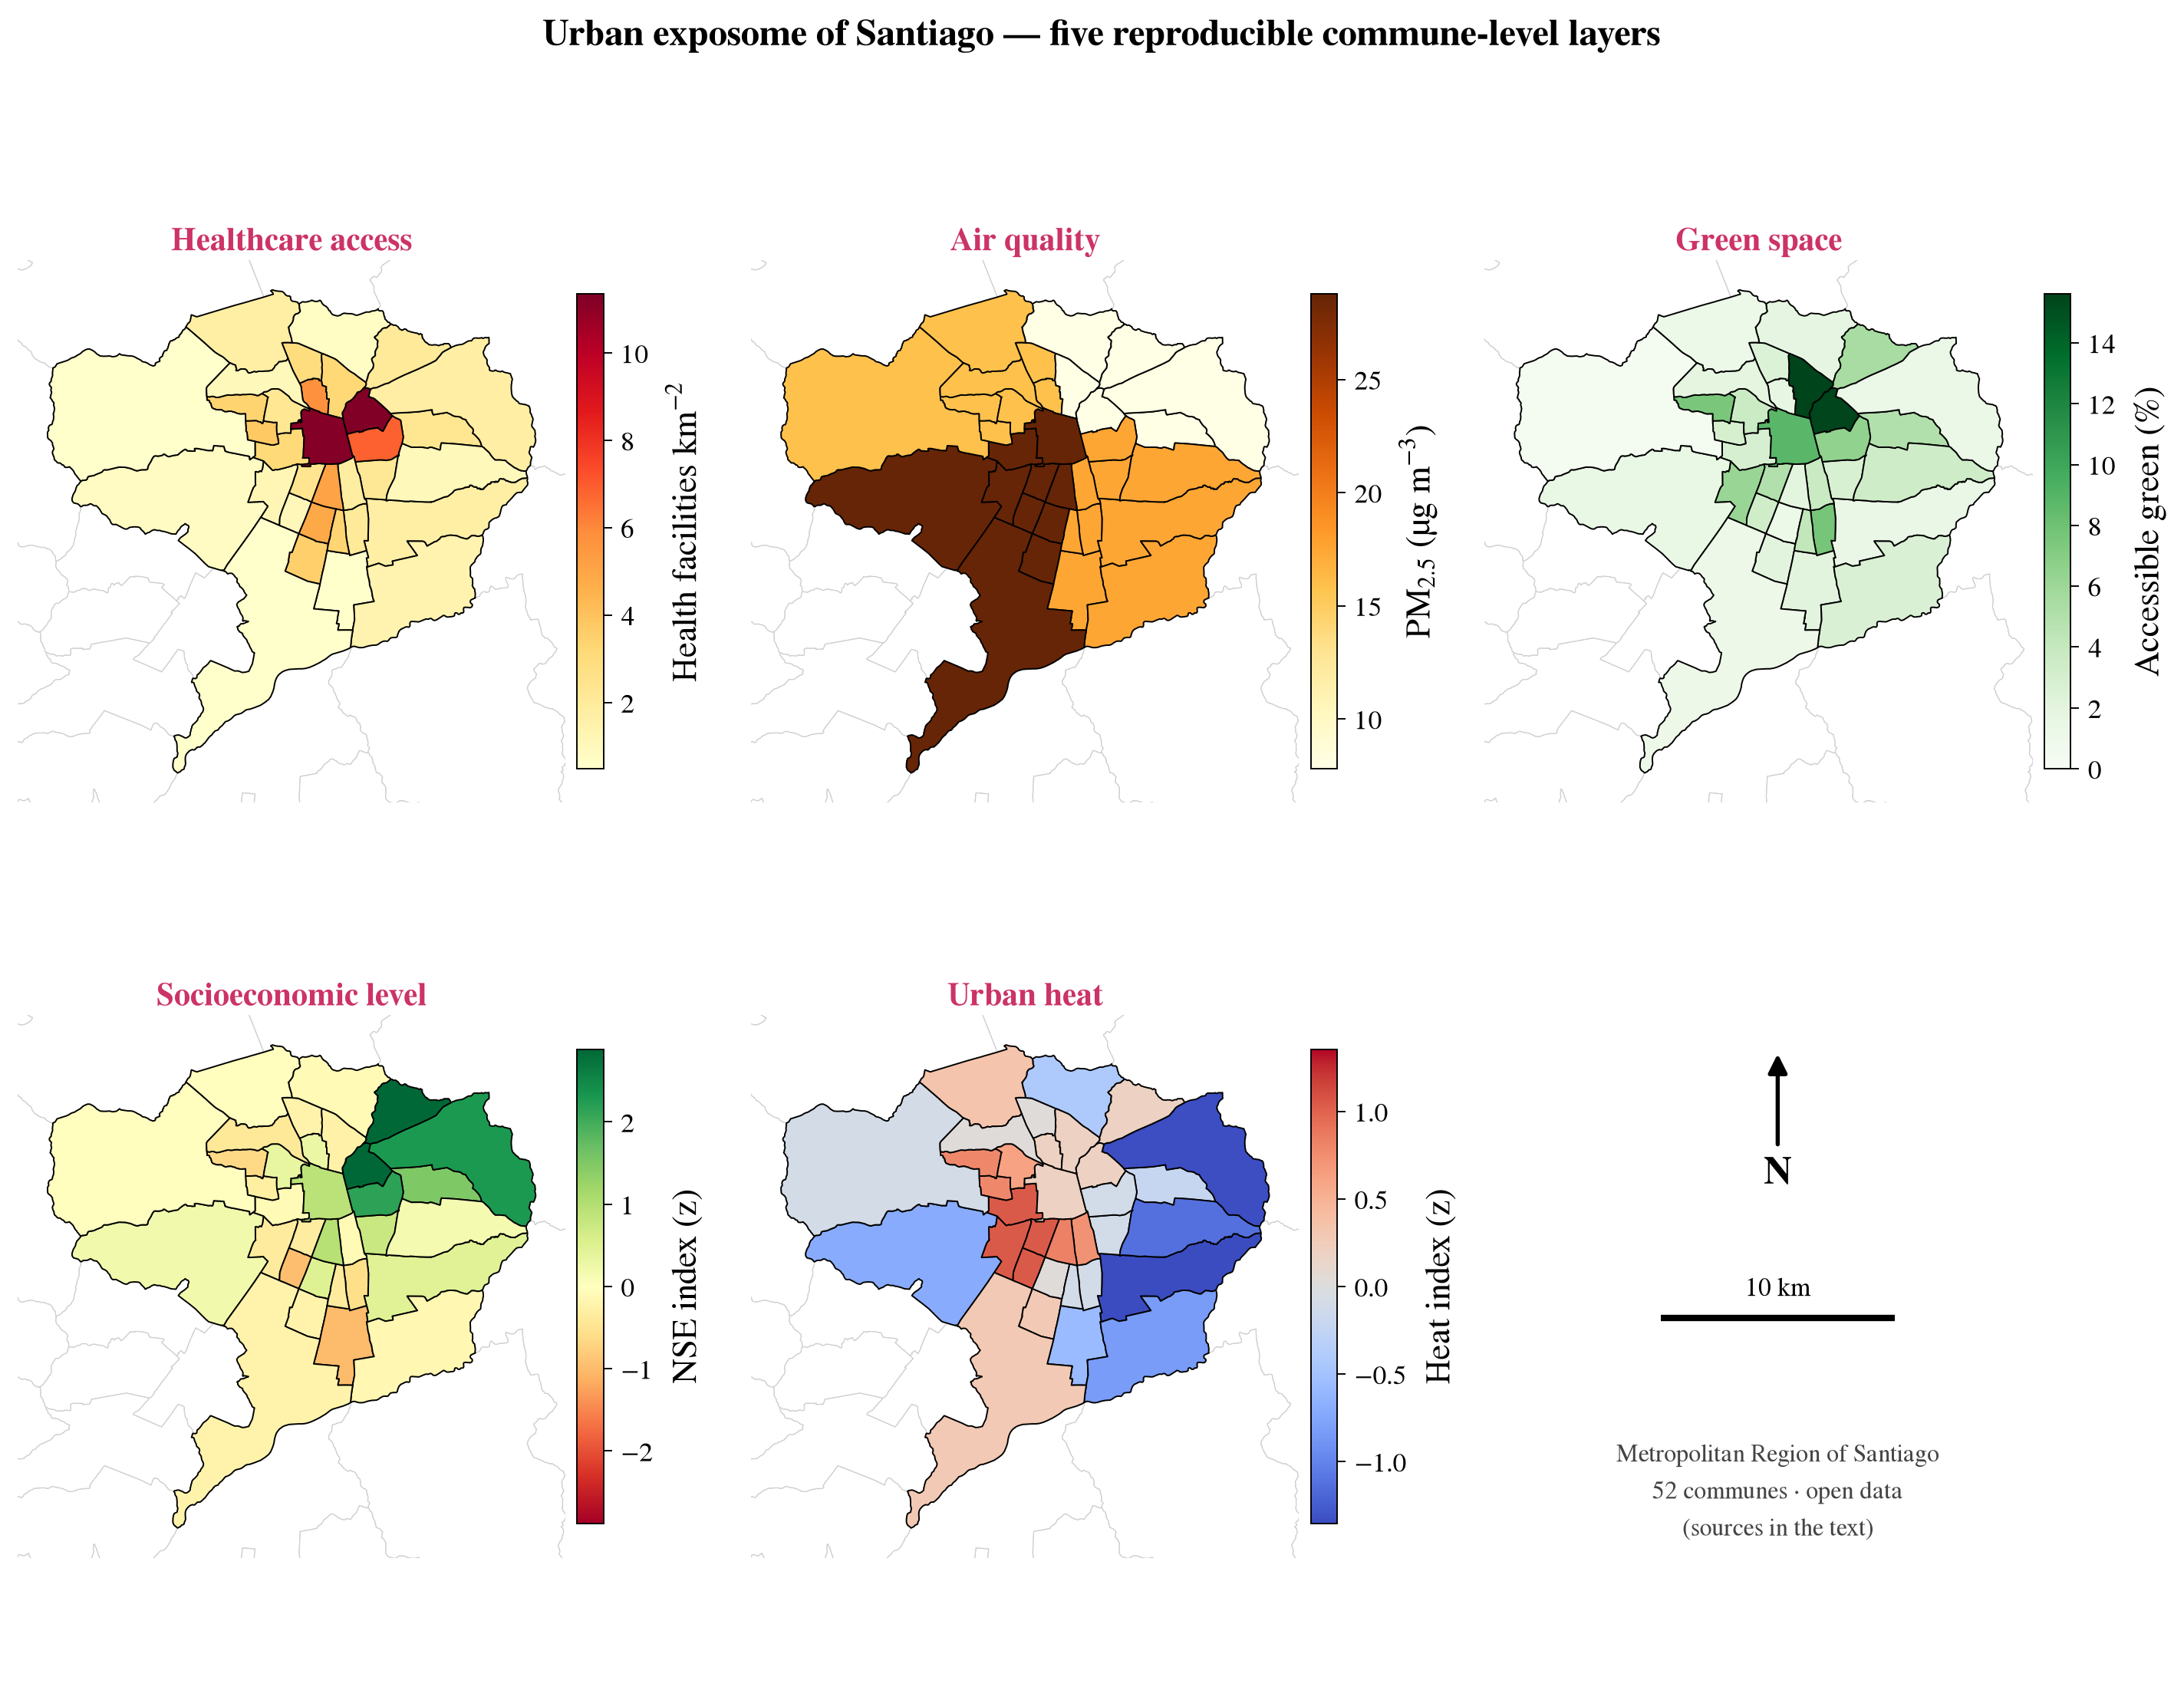
\includegraphics[width=\linewidth]{figures/exposome_5panel_santiago.png}
  \caption{\footnotesize Five commune-level exposome layers for the Metropolitan Region of Santiago, each harmonised to the same 52 communes. The colour scale of every panel and how it is computed are described in Section~\ref{sec:layers}. Diverging scales (socioeconomic level, urban heat) are standardised indices centred at the regional mean; sequential scales are physical magnitudes. The same east--west gradient recurs across panels: the high-income, leafy, cooler east versus the more polluted, hotter, lower-income centre and south-west.}
  \label{fig:fivepanel}
\end{figure}

\section{The five layers: indicator, computation and source}
\label{sec:layers}

For each layer I state \emph{what the colour scale represents}, \emph{how it is computed}, and \emph{the data source}.

\begin{description}[leftmargin=0pt,labelsep=0.4em,itemsep=4pt,style=nextline]

\item[\textcolor{softpink}{Healthcare access}]
\colorbarval{density of health facilities (establishments per km$^2$).}
Health amenities (hospital, clinic, pharmacy, doctors, dentist) are queried from OpenStreetMap, assigned to communes by spatial join, counted, and divided by the commune area in a metric projection (EPSG:32719); the notebook also derives mean / median / P90 distance to the nearest facility on an intra-commune grid. \emph{Source:} OpenStreetMap via OSMnx \citep{Boeing2017,OSM2024}.

\item[\textcolor{softpink}{Air quality}]
\colorbarval{annual-mean fine particulate matter PM$_{2.5}$ ($\mu$g\,m$^{-3}$).}
The CAMS atmospheric reanalysis is sampled on a $\sim$11\,km grid over the region (hourly, full year), averaged to an annual mean and aggregated to communes; values are benchmarked against the WHO 2021 annual guideline of 5\,$\mu$g\,m$^{-3}$ (every commune exceeds it). \emph{Source:} Open-Meteo Air-Quality API (CAMS), cross-checked against the official SINCA ground stations \citep{OpenMeteo2024,CAMS2024,WHO2021,SINCA2024}.

\item[\textcolor{softpink}{Green space}]
\colorbarval{share of the commune covered by accessible green space (\%).}
Parks, gardens, squares and recreation grounds are extracted from OpenStreetMap, dissolved into a single geometry (to avoid double counting), intersected with each commune, and divided by the commune area. Because this layer measures accessible, mapped green areas rather than total vegetation, Section~4 uses aerial-imagery computer vision to quantify the residual greenery that OpenStreetMap leaves out. \emph{Source:} OpenStreetMap \citep{OSM2024}.

\item[\textcolor{softpink}{Socioeconomic level}]
\colorbarval{composite socioeconomic index (standardised, regional mean $=0$).}
Per-commune household income and years of schooling (CASEN 2022) and the official small-area poverty estimate are each converted to $z$-scores; the index is the mean of income\,$(+)$, schooling\,$(+)$ and poverty\,$(-)$. \emph{Source:} Ministry of Social Development (CASEN, SAE poverty) via open data \citep{CASEN2022,OleaData2024}.

\item[\textcolor{softpink}{Urban heat}]
\colorbarval{heat-exposure index (standardised, regional mean $=0$).}
Daily 2024 temperatures are summarised per commune into summer mean $T_{\max}$, $T_{\max}$ P95, days $\geq$30/35\,$^\circ$C and tropical nights ($T_{\min}\geq$20\,$^\circ$C); these are $z$-scored and averaged. To avoid biasing large pre-Andean communes with uninhabited high-mountain pixels, the residential estimate uses only each commune's low-elevation (valley) band, identified with point elevations. \emph{Source:} Open-Meteo Historical Weather (ERA5-based reanalysis) \citep{OpenMeteo2024}.

\end{description}

\section{Integration and a first finding}

All five layers share the same 52 communes, so the master table supports immediate cross-analysis. A simple integration already yields a non-trivial result: socioeconomic level correlates \emph{significantly} with access to green space (Spearman $\rho\approx{+}0.44$, $p<0.001$) and to health services ($\rho\approx{+}0.59$, $p<0.001$), but \emph{not} with PM$_{2.5}$ ($\rho\approx{+}0.09$, $p\approx0.54$, n.s.) or NO$_2$ ($p\approx0.74$, n.s.); all are Spearman correlations with two-sided $p$-values over the $n{=}52$ communes (the critical $|\rho|$ for $p<0.05$ is $\approx0.27$). In Santiago, environmental inequity therefore operates mainly through unequal access to green space and services, while air pollution is governed more by the basin's topography and thermal inversion than by income --- exactly the kind of harmonised, multi-layer inference that exposome research at BrainLat requires.

\smallskip
{\centering
\small
\begin{tabular}{l c c c}
\hline
\textcolor{softpink}{\textbf{Layer vs.\ socioeconomic level}} & \textbf{$\rho$} & \textbf{$p$} & \\
\hline
Green space (\% accessible)   & $+0.44$ & $<0.001$ & *** \\
Healthcare facility density   & $+0.59$ & $<0.001$ & *** \\
Urban heat index              & $-0.14$ & $0.34$   & n.s. \\
PM$_{2.5}$ (annual mean)      & $+0.09$ & $0.54$   & n.s. \\
NO$_2$ (annual mean)          & $+0.05$ & $0.74$   & n.s. \\
\hline
\end{tabular}\par}
\smallskip
{\footnotesize Spearman rank correlations of each exposome layer against the composite socioeconomic index ($n=52$ communes; two-sided $p$-values; $|\rho|\gtrsim0.27$ is significant at $p<0.05$). *** $p<0.001$;\ n.s.\ = not significant. The two strongest, highly significant associations are social (green space, healthcare); the air-quality associations are not significant, consistent with a topographic rather than socioeconomic driver.}

\section{From an open baseline to satellite, time-domain exposure}

This demonstration is deliberately a \textbf{reproducible baseline}, not a finished product. Its most useful property is that it makes \emph{the incompleteness of current open samples visible} --- which is precisely where satellite Earth-observation data, and especially \textbf{time-domain} satellite data, add value:

\begin{itemize}[leftmargin=1.1cm,itemsep=2pt]
  \item \textbf{Green space.} OpenStreetMap maps \emph{public} parks but misses private gardens, street trees and seasonal vegetation, and under-represents affluent low-density areas. A computer-vision baseline on public aerial imagery --- the Excess Green index \citep{Woebbecke1995} thresholded with Otsu's method \citep{Otsu1979}, with a green-dominance test and morphological filtering to suppress false positives --- makes this concrete (Fig.~\ref{fig:cv}). \textbf{It detects substantially \emph{more} vegetation than the open layer --- of order $6$--$13\times$ in leafy residential sectors --- because $\sim$94\% of the detected greenery (private gardens and street trees) lies outside any OSM-mapped park.} Multispectral Sentinel-2 NDVI \citep{Sentinel2} extends this to full regional coverage and seasonality, and Landsat back decades.
  \item \textbf{Air quality and heat.} CAMS is a coarse ($\sim$11\,km) model field. Sentinel-5P (NO$_2$, aerosols) and Landsat/Sentinel-3 land-surface temperature resolve intra-urban gradients and the neighbourhood-scale urban heat island that a commune average smooths out \citep{Sentinel5P}.
  \item \textbf{Data completeness as a time-domain problem.} Treating the satellite archive as a time series lets us \emph{detect gaps, outliers and change} --- new parks, construction, deforestation --- and flag communes whose OpenStreetMap or model layers are stale or under-sampled. Earth observation thus becomes a quality-control layer over the open baseline, rather than a one-off snapshot.
\end{itemize}

\begin{figure}[h]
  \centering
  \includegraphics[width=0.84\linewidth]{figures/greenspace_cv_santiago.png}
  \caption{\footnotesize \textbf{Worked example --- detecting green space with computer vision.} A transparent pipeline --- Excess Green index \citep{Woebbecke1995} thresholded with Otsu's method \citep{Otsu1979}, plus a green-dominance test and morphological cleaning to suppress false positives --- outlines per-pixel vegetation (\textbf{lime}) on public aerial imagery. Overlaying the OpenStreetMap green polygons (\textbf{cyan}) shows that \textbf{$\sim$94\% of the detected vegetation in the residential sector lies outside any OSM-mapped park}: it is street trees and private gardens, absent from the OSM accessible-green layer that underlies the green file (Section~2). The contours track tree canopy and gardens, not roofs, streets or shadows. The same approach scales to CNN / foundation-model segmenters (SAM, DeepLabv3+) and to multispectral Sentinel-2 NDVI. \textit{Imagery © Esri, Maxar, Earthstar Geographics.}}
  \label{fig:cv}
\end{figure}

This is a direct transfer of my background in \textbf{time-domain astronomy} (multi-epoch light curves from ATLAS, ZTF and the Vera C.\ Rubin Observatory): multi-epoch calibration, gap and outlier handling, anomaly/change detection, and large heterogeneous data pipelines map one-to-one onto satellite revisit time series for exposome mapping. The computer-vision example above (vegetation segmentation on imagery) is the same competence applied to the spatial domain.

\section{Reproducibility}

The accompanying repository contains one notebook per factor, the master integration script (\texttt{scripts/build\_master\_exposome.py}), and a conda \texttt{environment.yml}. Every layer is harmonised to the 52 official communes of the Metropolitan Region (commune boundaries clipped to the regional limit), computed in a metric projection (EPSG:32719) and exported as both a table (CSV) and a GIS layer (GeoJSON), with a static map (PNG) and an interactive map (HTML). All inputs are open and require no authentication; a satellite (Google Earth Engine) appendix is provided as an optional extension. Each notebook also caches its raw API responses, so re-runs are offline and deterministic, and the master builder validates a strict one-to-one join (52 rows, no missing values) before writing.

\smallskip
\noindent\textbf{\textcolor{softpink}{Repository layout.}}
\begin{description}[leftmargin=0pt,labelsep=0.5em,itemsep=1.5pt,font=\ttfamily\small]
  \item[santiago\_\{healthcare\_access, air\_quality, green\_spaces,] \texttt{socioeconomic, climate\_heat\_exposure\}.ipynb} --- the five factor notebooks (one per exposome layer).
  \item[*\_exposome\_rm\_santiago.\{csv,geojson\}] per-factor commune indicators as a table and a GIS layer.
  \item[*\_santiago\_pub.png \textnormal{,} *\_santiago.html] publication-quality static map and interactive web map per factor.
  \item[scripts/build\_master\_exposome.py] joins all layers into \texttt{santiago\_exposome\_master.\{csv,geojson\}} ($52\times43$) with a metadata sidecar.
  \item[environment.yml \textnormal{,} README.md] reproducible conda environment and project documentation.
\end{description}

\printbibliography[title={Data sources and references}]

\end{document}
